\documentclass{article}

\usepackage[utf8]{inputenc}
\usepackage{graphicx}
%\usepackage{caption}
%\usepackage{subcaption}
%\usepackage{pdfpages}
%\usepackage{listings}
%\usepackage{soul}
%\usepackage{enumitem,amssymb}

\usepackage{color} %red, green, blue, yellow, cyan, magenta, black, white
\definecolor{mygreen}{RGB}{28,172,0} % color values Red, Green, Blue
\definecolor{mylilas}{RGB}{170,55,241}

% For Prof Evangelista to make comments
\usepackage[colorinlistoftodos]{todonotes}

% This version is also synced with a Github repository at
% https://github.com/devangel77b/ew496-sp2020-pak.git 
% and since I have the Overleaf professor edition we can also share it with
% more than two people (for example if Brooklyn Pritchard ever needs it. 

% biology style references
\usepackage[round,authoryear]{natbib}
\bibliographystyle{apalike}

\usepackage{fancyref}
% Evangelista note: should add amsmath and friends, listings if needed, hyperref for links and urls


% need a better title
\title{NEW TITLE PENDING}
\author{Alexis Pak}
\date{\today}

\begin{document}
\maketitle
\begin{abstract}
Some organisms rely on their antennae to determine the position or texture of objects around them and, more importantly, how to maneuver around them. Cockroaches (Blattidae) have tiny, hair-like sensors on their antennae that are connected to neurons that communicate messages to the brain. These messages are sent down their neural pathways in electrical activity called "spikes". This paper analyzes existing studies and determines how one could create a neural interface with a cockroach by stimulating spikes in its antennae. The product of this neural interface is understanding of and access to the cockroaches' motor skills, steering cockroaches left or right depending on the stimulation. The proximate aims of this project are to steer a cockroach and to evaluate the feasibility of a future lab exercise involving cyborg cockroaches. The ultimate aims are to learn neurophysiological and neuromechanical principles which may be applicable in restoring human function. 
\end{abstract}

% keywords: pick 3-5
{\scriptsize\textbf{Keywords:} cockroaches, Blattidae, neurophysiological, neuromechanical, steering}

\section{Introduction}

% Why is this topic important?

Although the human nervous system is very different from a cockroach’s, the structure and function of our individual neurons is actually very similar. This similarity allows us to learn about the human brain by studying cockroaches'. Invertebrates, including insects like cockroaches, are important model systems in neurophysiology because of their small, manageable size, the ability to easily access specific motor neurons that innervate entire specific muscle groups, and the presence of central pattern generators that produce locomotive behaviors. 


%On Mon, Nov 11, 2019 at 9:10 PM Alexis Pak <m215112@usna.edu> wrote:
%Good evening sir,
%
%It was good seeing you out in town today! I was thinking about the robo-roach project and was wondering what the applications (particularly military) of creating a robo-roach are? The project sounds really cool but I've been asking myself all weekend why I would want to wirelessly control a cockroach and can't seem to find a reason. I know they can definitely survive conditions that humans cannot, but what would they accomplish? Finding something? Spying on someone or something? Just some food for thought- I was wondering if you had any ideas! Thank you and have a great night.
%
%1. Spying. Have you seen the movie The Fifth Element? They glue a camera on a roach, and then use control to drive it to check something out. Otherwise in civilian science world they call this mission "search and recovery". 
%
%2. Neuromechanics / as a model system for other systems that are harder to work on. For example, imagine a patient with compromised neuromuscular control. The principles used to drive a roach around might be relevant for restoring function in such a patient. Alternatively, what is learned about roach control may transfer to other robot designs or control systems. Roaches are notable for _not_ controlling everything; they make use of passive mechanical feedback mechanisms to simplify the task of the neural controllers; this could allow for high performance parkour like robots in the future. Can you make the roach outperform the EW456 RC car? The base plant definitely does... The roaches can have much more invasive things done than we would ever do to a human patient during initial trials or basic research of a device, so such work is foundational for eventual applications like that. 
%
%#2 is the main reason there are entire labs that do cockroach neuromechanics. Google "Bob Full Berkeley lab" and "Tom Daniel UW lab" and "Ty Hedrick UNC lab" for example. We had speakers for biomechaincs seminar that work in this area - Jean Michel Mongeau (PSU) and Noah Cowan (JHU) and will have two more this week and next (Chen Li and Bo Cheng). Also check Simon Sponberg Georgia Tech; Shai Revzen and Talia Moore (Michigan). 
%
%If there's other things you'd like to try during 282D or 496 (whichever) then we can make room for that too. Backyard Brains is just one thing I want to try in the spring to see how accessible it is for mids, possibly use it in future course offerings, or as something a motivated mid could build a project around.





% Literature Review
Many people have already conducted research on and tested the feasibility of steering a cockroach using electrical stimulation. \citet{moore1998directed} were able to ``drive'' Slovenian cockroaches through a zig-zagged track. They found that, although results varied, only a small fraction of the cockroaches responded and were consistently sensitive to the stimuli \citep{moore1998directed}. They also discovered that, in most cases, current directed toward the base of an antenna resulted in faster forward motion whereas current directed further down the antenna resulted in slow walking, halting, and even reverse motion \citep{moore1998directed}.

A more detailed study of higher neural structures showed that, the central complex, a part of the arthropod brain that receives sensory information and outputs to premotor regions, supervises locomotion \citep{guo2013neural}. \citet{guo2013neural} performed the same type of experiment as \citet{moore1998directed}, but also created firing maps based on the roaches' continuously changing speed and direction, which demonstrated that many of the central complex units they recorded were tuned to particular turning and forward walking speeds.

Like the previous two experiments, \citet{holzer1997locomotion} also applied electrical stimulation of nerves using an electronic backpack. Unlike the previous experiments, however, they recorded their measurements on a styrofoam trackball connected to a computer, which allowed them to record the turning rate and forward movement in response to stimulation to the roach's antennae \citep{holzer1997locomotion}. Their experiments also showed that, despite large variance, they could achieve directional locomotion control by stimulating the nerves of cockroaches' antennae.

\citet{whitmire2013kinect} demonstrated how engineering can be used to steer cockroaches by adding external computer vision, making the application of electrical stimulus autonomous. By observing successful trials of cockroach steering, the team found that the deviation from the prescribed path and the net angular change and velocity when turning could be used to create a quantitative analysis of the experiment \citep{whitmire2013kinect}. Unlike the previous study, which required a human operator to manually stimulate with a remote control, this one steered the roaches using a computer vision platform that automatically stimulates the roaches \citep{whitmire2013kinect}. The computer vision platform allowed for automated variation in stimulation patterns as the cockroach adjusted its path \citep{whitmire2013kinect}. From the quantitative analysis, the team was able to get a precise estimate of the effects of each stimulus, allowing the to optimize the efficacy of their stimulation technique \citep{whitmire2013kinect}. 





% What do I intend to do, hypothesize, etc?

Based on the findings of these previous experiments, I intend to replicate their experiments to evaluate the feasibility of a future lab exercise involving cyborg cockroaches. My ultimate aim of steering a cockroach is to learn about neurophysiological and neuromechanical principles which may be applicable in restoring human function. I hypothesize that that there will be large variance in results and less than 25\% of trials will be successful, but the successful trials will demonstrate that stimulation of the left antenna will steer the cockroach right and vice versa for the opposite antenna. I also hypothesize that, for the cockroaches that do respond, more current will result in sharper and wider turns.







 %\section{Introduction}
\section{Methods and materials}
 %\section{Methods and Materials}
\section{Results}

%For results talk about what you would measure.

To determine the results of the experiment, I would conduct the experiment on each cockroach. Ideally, I would have at least 10 cockroaches to test on. For each experiment, I would use a timer to measure the time it took for a cockroach to react to the stimulation and the electrical tape to measure the angle of turn. 

% What else should I measure?

With the cockroaches that successfully turn left and right when stimulated, I will place them on track made of thin strips of electrical tape consisting of straight paths and \ang{90} turns and observe their ability to make it all the way through. I will also test the roach's ability to turn to various angles by modulating the current sent to its antennae and evaluating its performance of different maneuvers such as the Dieudonne Spiral, a zig-zag, and a sinusoid. % talk more about how it would execute the different maneuvers 

Once directional control is achieved, I will try to achieve speed control. Stimulation to the antennae may not necessarily control speed in addition to direction, so I will attempt to stimulate other areas of the roach's body to change its speed.

{\begin{figure}[ht!]
\centering
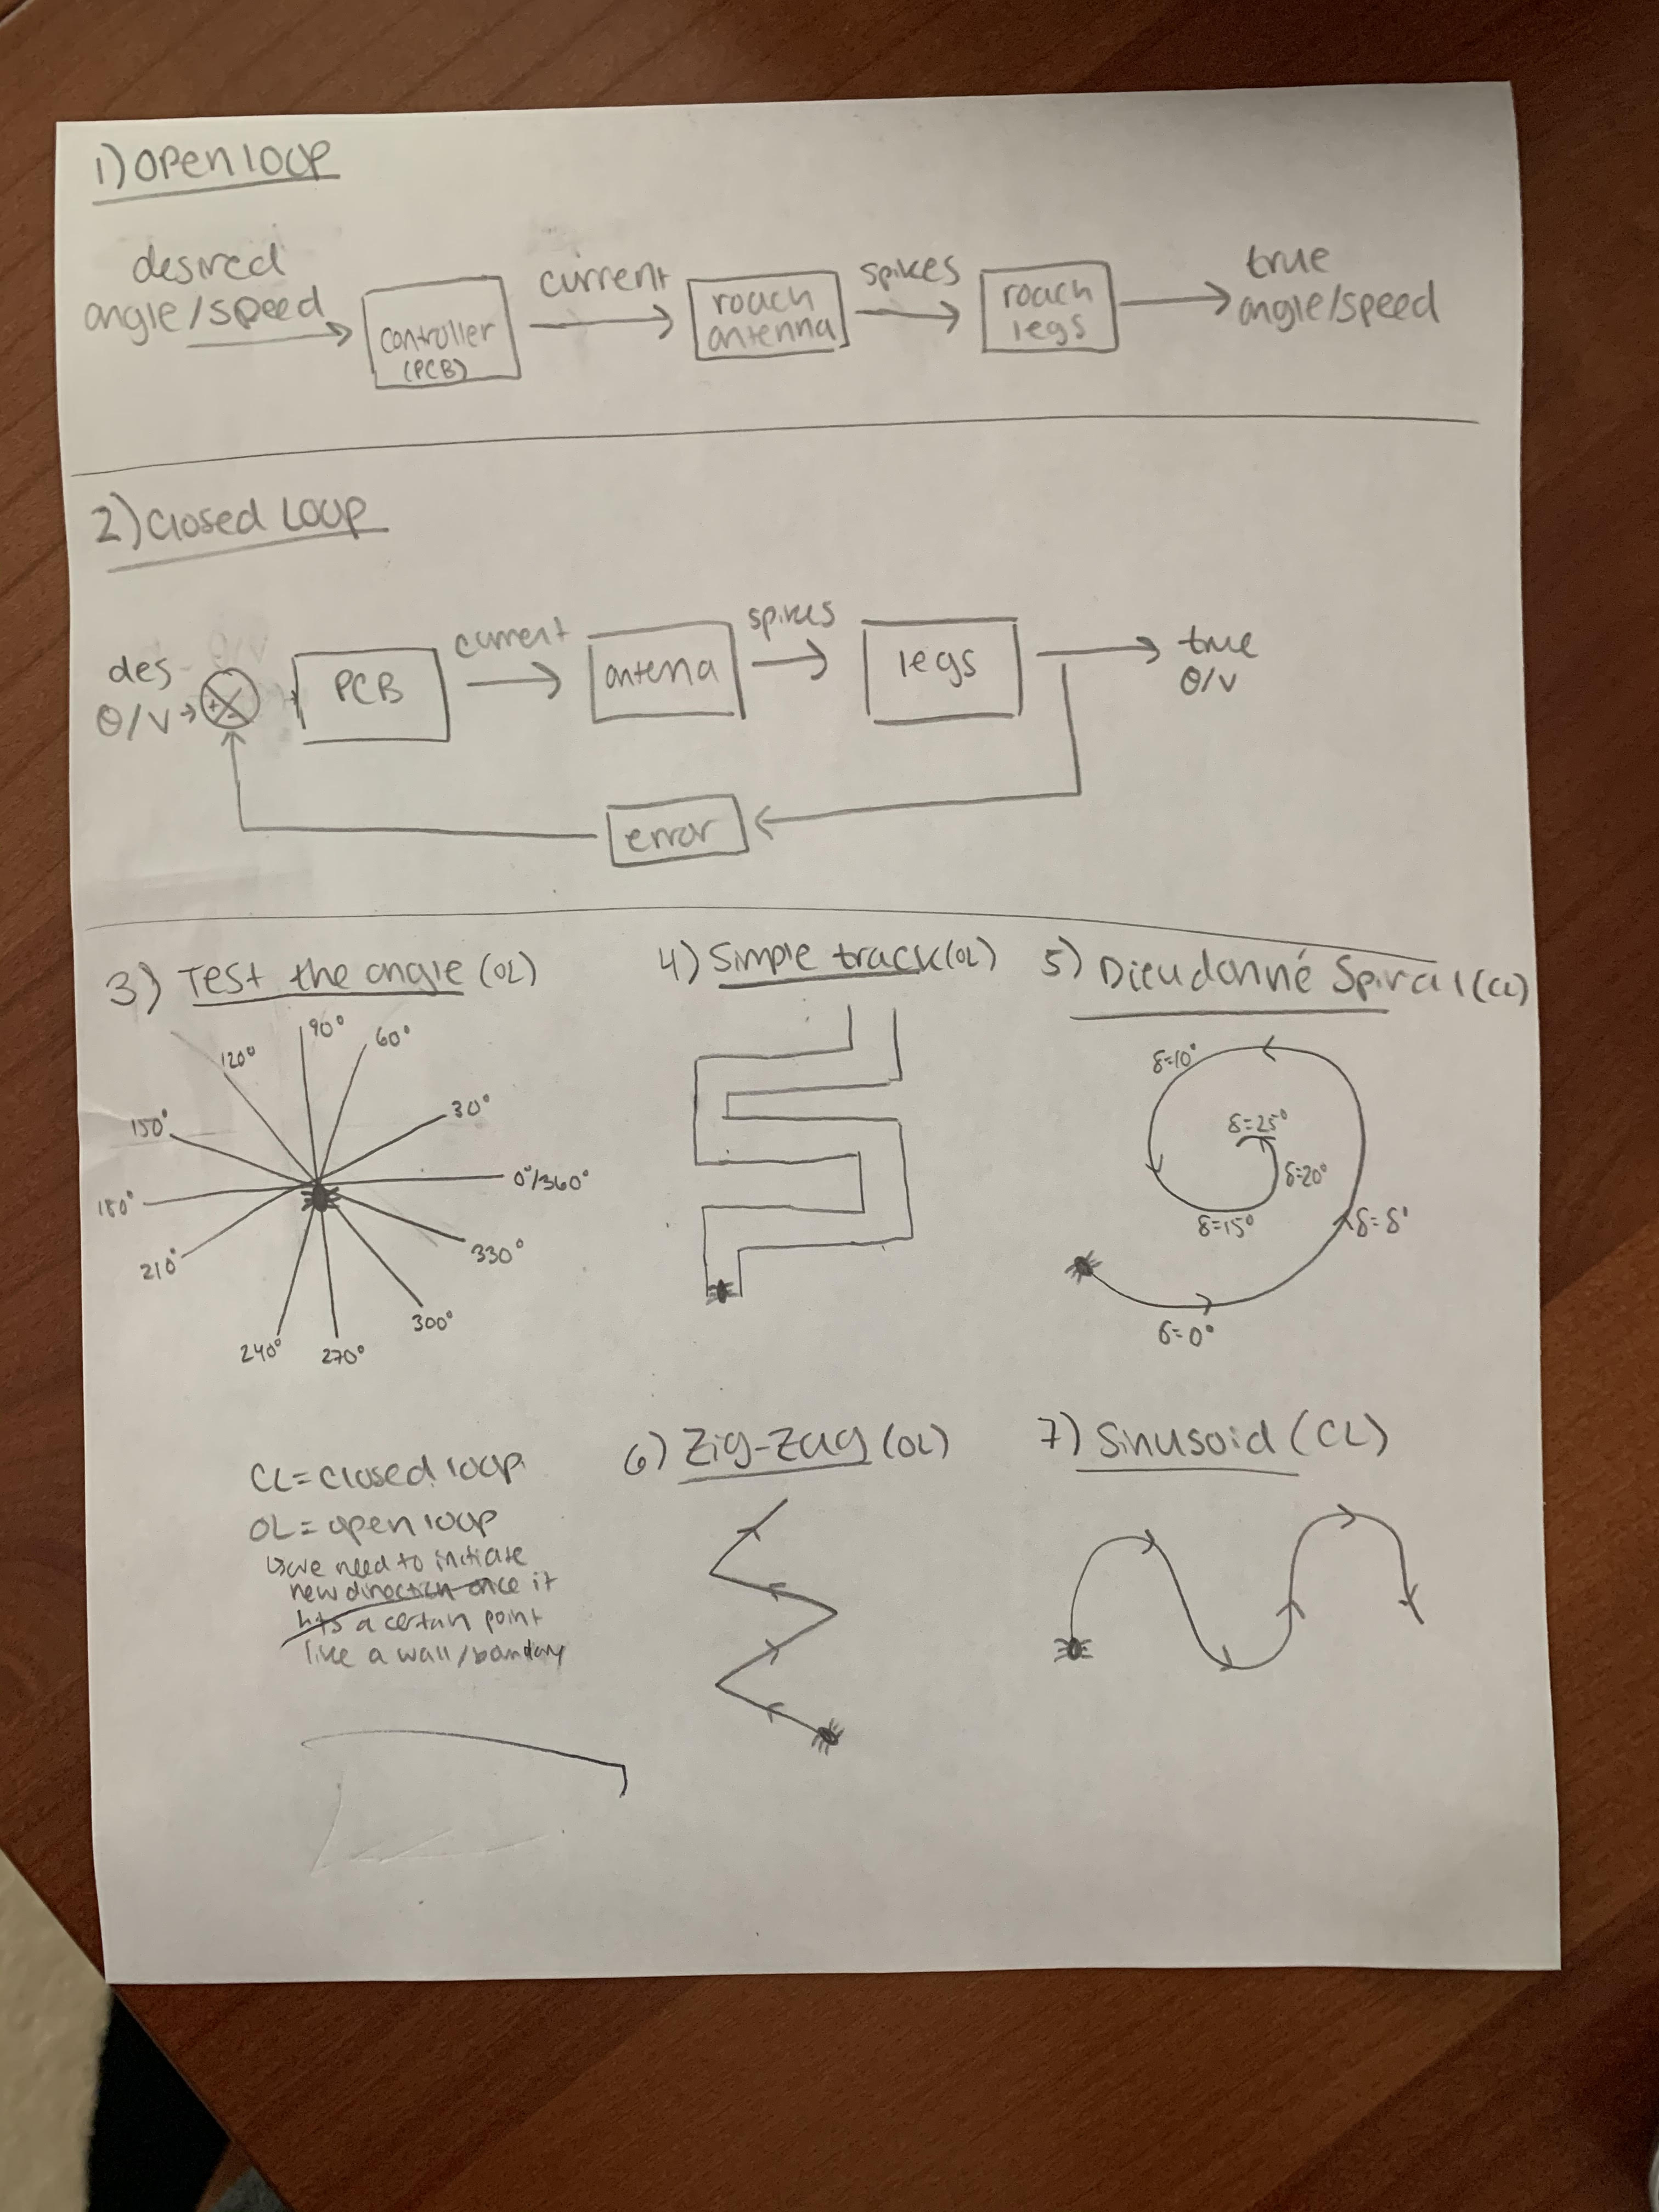
\includegraphics[scale=0.1]{Figures/OpenClosedLoops.jpg}
\caption{Rough ideas...feedback please?}
\label{fig:rough}
\end{figure}}


  %\section{Results}
\section{Discussion}

% What is the significance of the things I will measure?

By measuring the time, current, and angles of turn throughout different maneuvers, I can quantify the directional and speed behavior of the cockroach. Using this relationship between applied current and speed or direction, I can achieve full remote control over the cockroach's movement. 

Being able to remotely control a cockroach is useful for a couple of reasons. The first is spying and surveillance. By equipping a camera onto a roach, humans can use control to drive it and investigate a scene. Some papers have written about possible search and recovery missions, using cockroaches to find possible survivors so that humans are not looking aimlessly or putting themselves at risk when they are searching for survivors. The second reason is the simplified model. Because cockroaches have similar neurons to humans but are much less complex organisms, they can serve as a neuromechanical model system for complex organisms like humans. The principles used to steer a cockroach could be relevant to restoring function in a patient with compromised neuromuscular control. The third reason is control systems and design. What is learned about cockroach control may transfer to other robot designs or control systems. Cockroaches make use of passive mechanical feedback mechanisms to simplify the task of the neural controllers, which allows for high performance parkour. If we can understand and control a cockroach's neural interface with locomotion, we could potentially make it outperform an RC car or other bot. %\section{Discussion}

\section{Acknowledgments}
I thank a Brooklyn Pritchard, Sofia Figueroa, Cameron Smith, and John Trombetta for comments and discussion that helped my thinking on this topic; (others?)...

% References
\bibliography{pak.bib}
\end{document}









